%--------------------------------------------------------------------------
\chapter{INTRODUCTION}

\vspace{3em}
\setlength{\epigraphwidth}{0.86\textwidth}
\setlength{\epigraphrule}{0pt}
\epigraph{
	\textit{Music has become an almost arbitrary matter, and composers will no longer be bound by laws and rules, but avoid the names of School and Law as they would Death itself...}
}{\vspace{2em}-- Johann Joseph Fux}
\vspace{1em}

%--------------------------------------------------------------------------
\section{Derivation and Polyphony}

\begin{figure}[htbp]
    \centering
	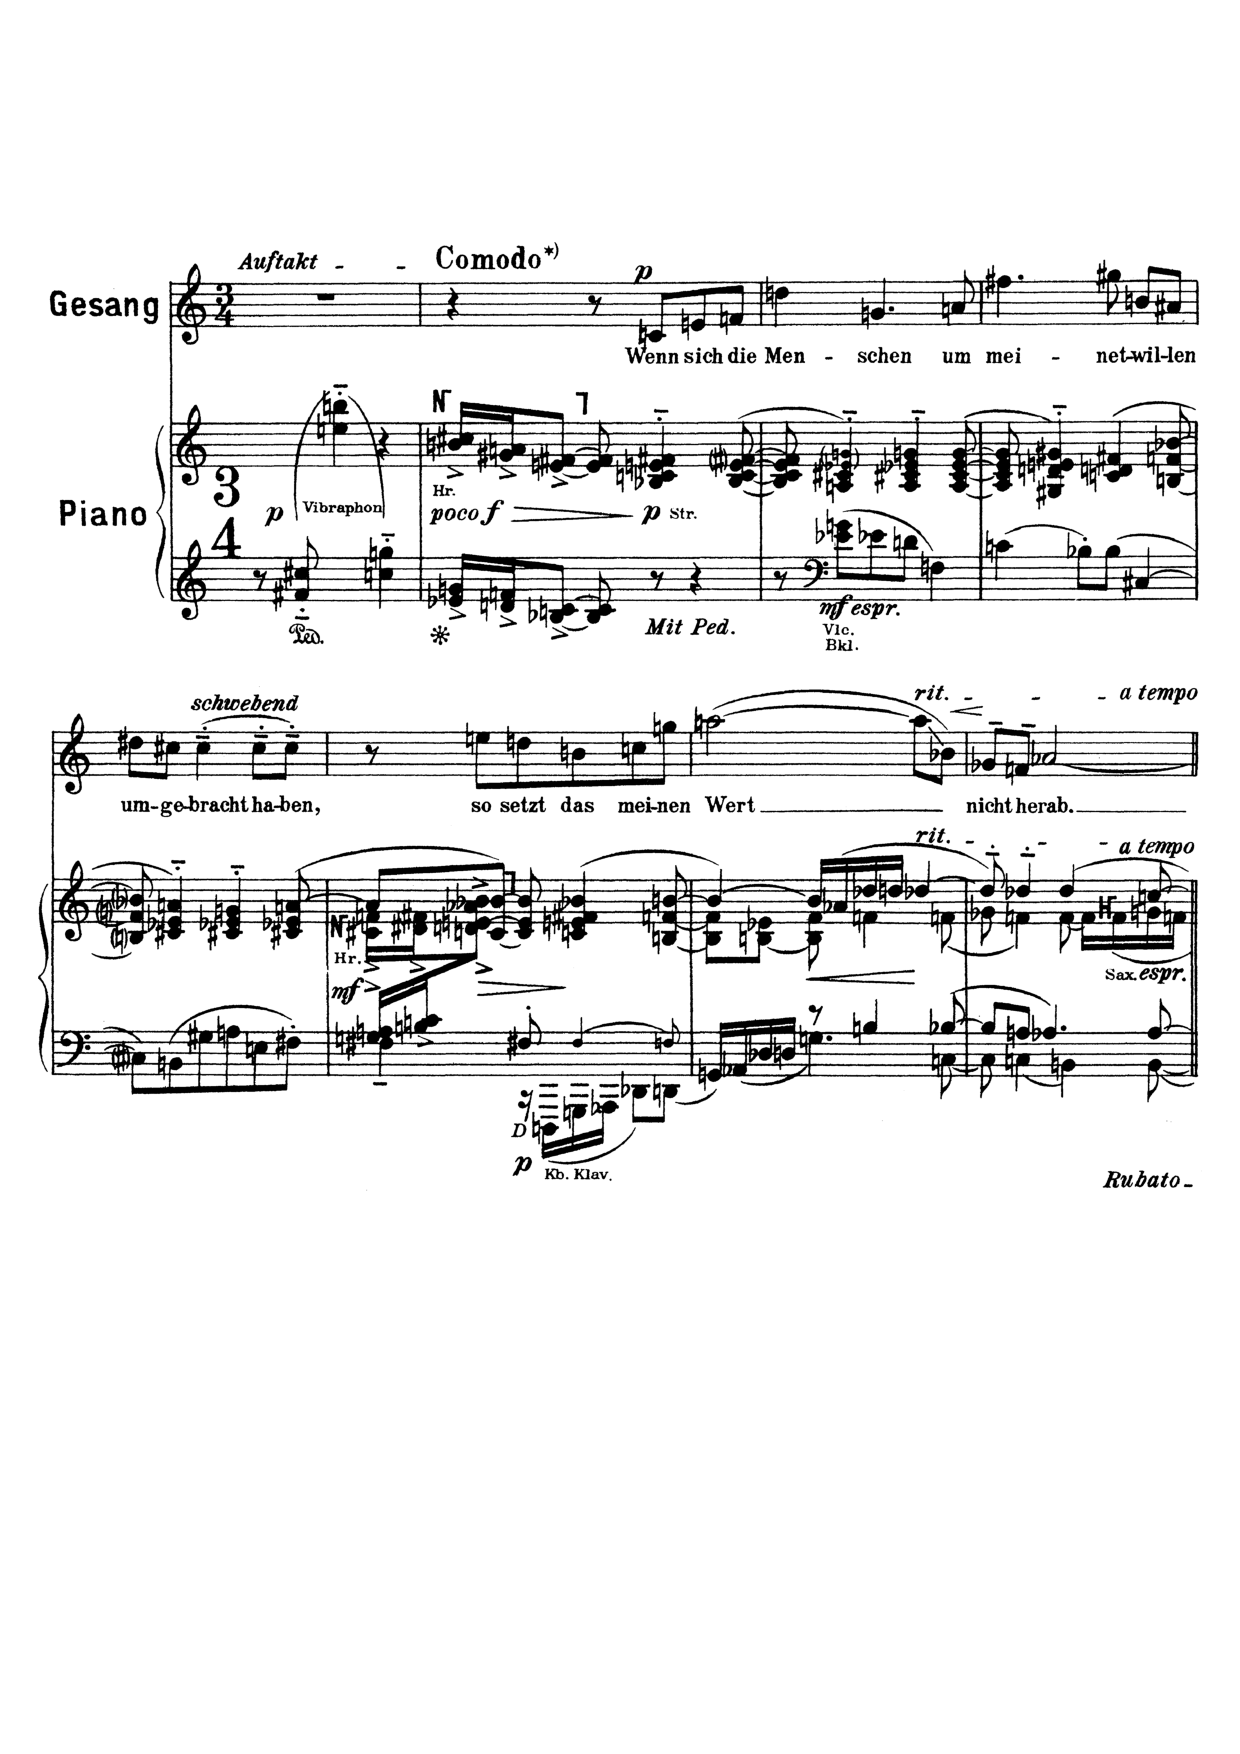
\includegraphics[width=6.5in]{figures/berg1.pdf}
	\caption[Berg's \emph{Lulu}]{Alban Berg's \emph{Lulu} \cite[182]{Starr1984}.}
	\label{fig:berg-lulu}
\end{figure}

Derivation is the process of extracting ordered segments from rows in order to generate new compositional materials. It is a technique that dates back to the Second Viennese School. In its most incipient form, a composer may simply extract these segments from a row, and combine them to form another, as we see in Berg's \emph{Lulu}. The basic row used by Berg is $S = \{ 10, 2, 3, 0, 5, 7, 4, 6, 9, 8, 1, 11 \}$. In the Prologue, however, one is greeted with the row $\{ 10, 3, 4, 9, 2, 7, 8, 1, 0, 5, 6, 11 \}$, as depicted in Fig.~\ref{fig:berg-prologue}. It is clear that the segments that constitute the Prologue's row are ordered segments in the basic row form, and the fact that one row cannot obtained from another via row operations is irrelevant.

%\begin{figure}[htbp]
%\begin{music}
%\nostartrule
%\startextract
%\NOTes\nq{_bd_ecfge^fh^g^ji}\en
%\setemptybar
%\endextract
%\end{music}
%\caption[Berg's \emph{Lulu} Basic Row]{Basic row in Alban Berg's \emph{Lulu} \cite[182]{Starr1984}.}
%\label{fig:berg}
%\end{figure}
%
%\begin{figure}[htbp]
%\begin{music}
%\nostartrule
%\startextract
%\NOTes\Qqbu{_b}{_e}{=e}{h}\Qqbu{d}{g}{^g}{^j}
%\Qqbu{c}{f}{^f}{i}\en
%\setemptybar
%\endextract
%\end{music}
%\caption[Berg's \emph{Lulu} Derived Row]{Derived row in Alban Berg's \emph{Lulu} \cite[182]{Starr1984}.}
%\label{fig:berg2}
%\end{figure}

\begin{figure}[htbp]
    \centering
	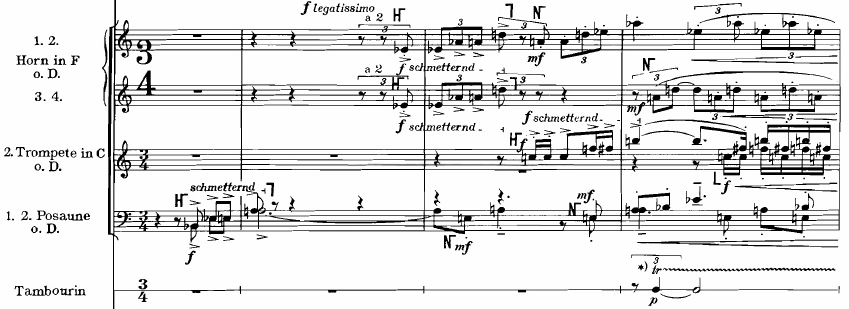
\includegraphics[width=6.5in]{figures/berg2.png}
	\caption[Derived Row in Berg's \emph{Lulu}]{Derived rows in the \emph{Prologue} of Alban Berg's \emph{Lulu} \cite[182]{Starr1984}.}
	\label{fig:berg-prologue}
\end{figure}

Less naive approaches to derivation ofted involve a derived row that will have more structure. In them, one will often see a combination matrix where derived and original rows are matched with some tewlve-tone or order operation of themselves, or both. This is illustrated in Ex.~\ref{ex:derivation}.

\begin{example}
\label{ex:derivation}
We may use the basic row in \emph{Lulu} as motivation for a basic derivation procedure. The first step is to create a $2 \times 24$ array where the first row is $S$ followed by $\R \circ S$, and the second row is initially undefined.
\begin{equation}
    \left[
    \begin{array}{cccccccccccc|cccccccccccc}
        10 & 2 & 3 & 0 & 5 & 7 & 4 & 6 & 9 & 8 & 1 & 11 & 11 & 1 & 8 & 9 & 6 & 4 & 7 & 5 & 0 & 3 & 2 & 10 \\
        . & . & . & . & . & . & . & . & . & . & . & . & . & . & . & . & . & . & . & . & . & . & . & .
    \end{array}
    \right] \enspace.
\end{equation}
Next, one chooses an arbitrary segment, and separates it from the the top row by placing in in the bottom row:
\begin{equation}
    \left[
    \begin{array}{cccccccccccc|cccccccccccc}
        . & 2 & 3 & . & . & . & 4 & 6 & 9 & 8 & 1 & 11 & . & . & . & . & . & . & 7 & 5 & 0 & . & . & 10 \\
        10 & . & . & 0 & 5 & 7 & . & . & . & . & . & . & 11 & 1 & 8 & 9 & 6 & 4 & . & . & . & 3 & 2 & .
    \end{array}
    \right] \enspace.
\end{equation}
Let $T = \{ 10, 3, 4, 6, 9, 8, 1, 11, 7, 5, 0, 2 \}$. Then $T$ is a row derived from $S$. In particular, the ordered segment $\{ 10, 0, 5, 7 \}$ in $S$ is preserved by $\R \circ T$.
\end{example}

It is of interest to note at this point that, in this kind of construction, the choice of a particular segment is already an important compositional decision. This choice bears relevance in that it extablishes motivic material, that is, the segment itself. It also potentially introduces complementary harmonic regions, one given by the segment, the other given by its set complement. Moreover, and perhaps more importantly, it presents an opportunity for exploring syntax. There are a multitude of ways in which a composer may obtain syntax from a simple derivation procedure such as the one given in the example above. One way would be to find an operation that makes the chosen segment invariant. In particular, it is easily checked that $S_1 = \{ 10, 0, 5, 7 \} = \R\T_5\I \circ S_1$. One can then extend Ex.~\ref{ex:derivation} into the combination array $[S \; | \; R \circ S \; | \; \R\T_5\I \circ S \; | \; T_5\I \circ S_1]$. In the extended array, the segment $S_1$ would be preserved, but the row derived from $\R\T_5\I \circ S$ would not be a transform of $T$. If the set complement of $S_1$ in $T$ were parsed to produce more than one harmonic region, then the complement of $S_1$ under this new derived row would produce different harmonic regions. This can be very pertinent compositionally, as one would be capable of producing contrasting harmonic regions while maintaining motivic coherence under the $S_1$ segment.

Yet another way of generating syntax from derivation would be to follow $S$ with $T$ itself. One would then derive a new row from $T$, say $Q$, and eventually follow $T$ with $Q$. Repeating this procedure \emph{ad libitum} could generate many contrasting harmonic regions. In particular, this tipe of derivation is seen in Donald Martino's \emph{Notturno} of 1974, a composition that won the Pulitzer Prize in the following year \cite[181]{Starr1984}. If, by compostional choice, the chain of derived rows picked always the same order numbers, then a potential for rhythmic and agogic coherence could also be explored.

In one of the seminal academic works in the field of 12-tone theory, \cite{Starr1984} utilizes a mostly set-theoretic framework to understand and categorize rows and procedures involved in producing derivation, polyphony, and self-derived combination matrices. The main objective is similar to ours, in it has a bias toward unveiling self derivation, which unfortunately still remains a somewhat obscure topic. The set-theoretic approach revolves around the idea of looking at collections from the standpoint of their order constraints: a totally constrained set with no precedence contradictions is a 12-tone row; a completely unconstrained set of 12 tones represents the free aggregate; a maximally constrained one is what the author calls the simmultaneous aggregate, that is, a 12-tone cluster. Sets that live in between can often be projected in the middle and background of a composition, fact that amounts to a Schenkerian-flavored view of the whole process.

Mathematically, the ideas in \cite{Starr1984} translate into considering the set $U$ of all ordered pairs of pitch classes. There are 12 choices for the first position, and 12 choices for the second position. As both choices are independent, this set has cardinality $12^2 = 144$. An element of $U$ is called an order constraint, and a subset $C$ of $U$ is called a pitch-class relation. The latter can be viewed as a $12 \times 12$ matrix where the entry $c_{ij}$ is equal to one whenever $\{ i, j \} \in C$, and zero otherwise. One can the apply biwise operations to these matrices in a very computationally efficient manner: bitwise \emph{and} and \emph{or} correspond respectively to set intersection and union. For any pitch classes $x$ and $y$, we define a relation $x \sim y$ on the power set of $U$ by the set inclusion of the element $\{ x, y \}$. A subset $C$ will then be reflexive if, whenever an element of $C$ (which is a set) contains the pitch class $x$, then $\{ x, x \} \in C$. In words, reflexivity means that if a reflexive collection $C$ of notes contains an element $x$, then $x$ precedes (and follows) itself in $C$. The free aggregate is a minimal reflexive subset of $U$ that contains all 12 tones. The relation $\sim$ will be symmetric if $\{ x, y \} \in C$ implies $\{ y, x \} \in C$, and antisymmetric whenever $\{ x, y \} \in C$ implies $\{ y, x \} \notin C$, for $x \ne y \in \mathbb{Z}/ 12 \mathbb{Z}$. Similarly, transitivity is defined as $\{ x, y \} \in C$ and $\{ y, z \} \in C$, then $\{ x, z\} \in C$; and trichotomy is defined as either $\{ x, y \} \in C$ or $\{ y, x \} \in C$ for any $x \ne y \in \mathbb{Z}/ 12 \mathbb{Z}$. The relation $\sim$ is, of course, an order relation on the set of 12 tones by definition. A partial order is one that is reflexive, transitive, and antisymmetric, while a total order (a row), is a partial order that satisfies trichotomy.

Often, pitch-class relations will contain many redundancies due to transitivity. In order to express these relations as oriented graphs, one must first remove, or prune such redundancies. This process can be reversed and a pitch-class relation can be extended to the point of its transitive closure. It is also common for a pitch-class relation to be absent of any order constraint involving both $\{ x, y \}$, in which case we say $x$ and $y$ are incomparable. Such $x$ and $y$ are bound to be struck together, or else be \emph{linearized} by the injection of some constraint that will make them comparable, as long as the is still a partial order, that is, as long as it does not introduce a symmetry, for instance. The set of all total orderings that can be linearized out of some partial order is called its total order class. In a completely analogous manner, one can \emph{verticalize} a pitch-class relation by removing constraints, and again minding that the result is still transitive and symmetric. We say a partial order covers another whenever the former is a verticalization of the latter. A simple procedure to guarantee that a verticalization will remain a partial order is to take its union with the free aggregate, then subject this union to an extension operation, thus providing reflexivity in the first step, as well as transitivity in the second. We can say the following about covering and about unions and intersections of pitch-class relations:

\begin{theorem}
    \cite[193]{Starr1984}
    \begin{enumerate}[i.]
        \item Covering is transitive;
        \item A pitch-class relation is covered by its extension;
        \item If a pitch-class relation covers another, then the extension of the former covers the extension of the latter.
    \end{enumerate}
\end{theorem}

\begin{theorem}
    \cite[194]{Starr1984}
    Let $A$ and $B$ be partial orders and denote by $\Toc(A)$ and $\Toc(B)$ their respective total order classes. Then
    \begin{equation}
        \Toc(A) \cap \Toc(B) = \Toc(\Ext(A \cup B)) \enspace,
    \end{equation}
    where $\Ext$ is the extension operator.
\end{theorem}

\begin{theorem}
    \cite[194]{Starr1984}
    The intersection of two partial orders is again a partial order.
\end{theorem}

Of vital importance is the fact that one can operate on pitch-class relations the same way one operates on pitch-class sets:

\begin{theorem}
    \cite[195]{Starr1984}
    Let $C$ be a pitch-class relation and $\{ a, b \}$ an element of $U$ such that $\{ a, b \} \in C$.
    \begin{enumerate}[i.]
        \item If $F$ is a pitch-class operation, then $\{ F(a), F(b) \} \in F(C)$ if and only if $\{ a, b \} \in C$. In particular, if $R(C)$ is the retrograde of $C$, then $\{ a, b \} \in R(C)$ if and only if $\{ b, a \} \in C$.
        \item If $C$ is totally ordered, then $R(C) = (S \setminus D) \cup F$, where $S$ is the simultaneous aggregate and $F$ is the free aggregrate.
        \item If $C_1$ covers $C_2$, then $F(C_1)$ covers $F(C_2)$.
        \item Finally, if $C$ is $FR$-invariant, then all cycles in $F$ have length two.
    \end{enumerate}
\end{theorem}

%--------------------------------------------------------------------------
\subsection{Aggregate Realizations}

\begin{figure}[htbp]
    \centering
	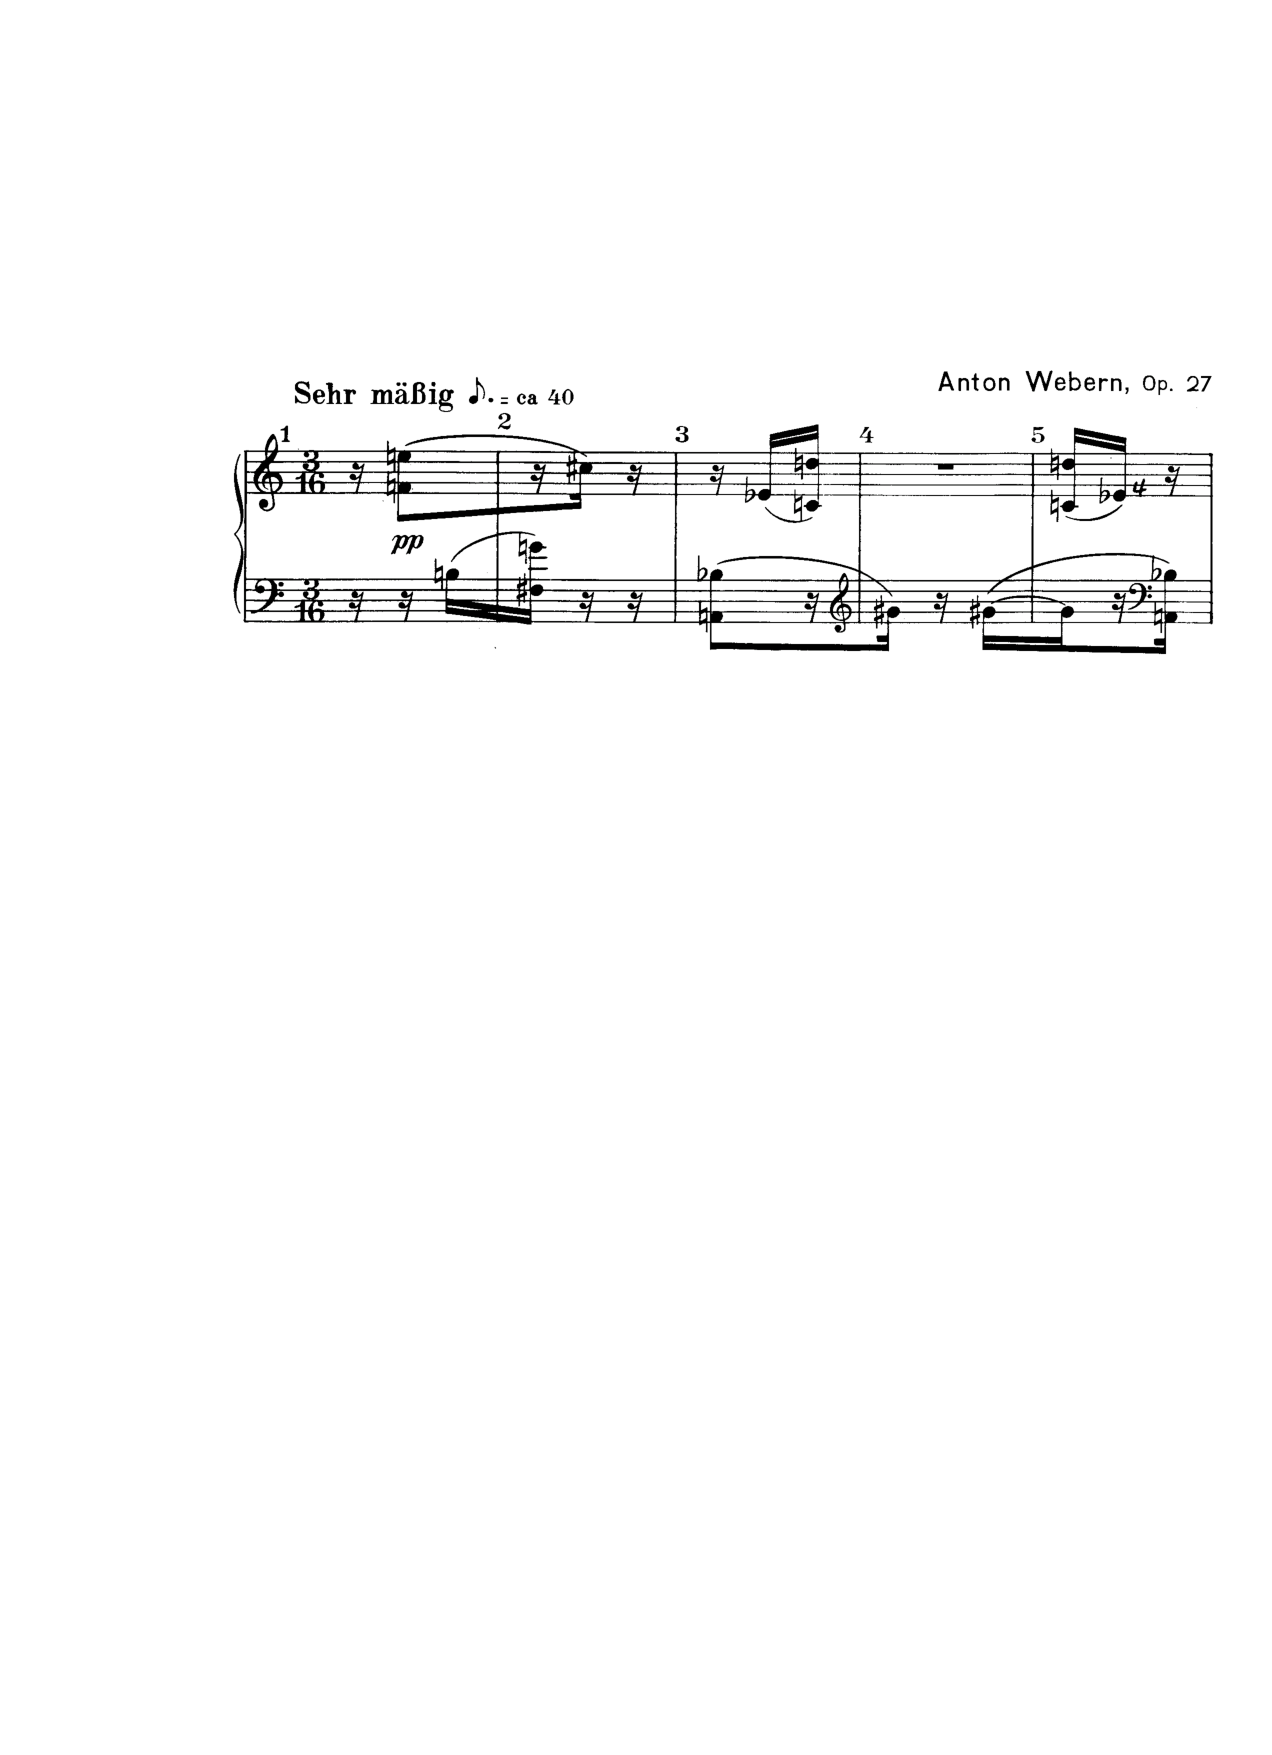
\includegraphics[width=6.5in]{figures/webern1.pdf}
	\caption[Bars 1--7 in Webern's Op.~27]{The initial bars in Webern's Op.~27.}
    \label{fig:webern-27}
\end{figure}

In this section we will define the important concept of \emph{aggregate realizations}, which will, in turn, lead to a classification of partial orders, as well as to many musical applications. An aggregate realization is a particular type of partial order $C$ in which, for any pair of pitch classes $a, b$, if $a$ and $b$ are incomparable in $C$, then the set of pitch classes that preceed $a$ in $C$ is equal to the set of pitch classes that preceed $b$ in $C$, and also the set of pitch classes that follow $a$ in $C$ is equal to the set of pitch classes that follow $b$ in $C$.

\begin{figure}[htbp]
    \centering
	\begin{tikzcd}
        & E \arrow[dr] && G \arrow[dr] && B\flat \arrow[dr] && D \arrow[dr] & \\
        * \arrow[dr] \arrow[ur] && B \arrow[dr] \arrow[ur] && C\sharp \arrow[dr] \arrow[ur] && E\flat \arrow[dr] \arrow[ur] && G\sharp \\
        & F \arrow[ur] && F\sharp \arrow[ur] && A \arrow[ur] && C \arrow[ur] &
    \end{tikzcd}
	\caption[Aggregate Realization of Bars 1--7 in Webern's Op.~27]{An aggregate realization of the initial bars in Webern's Op.~27. At its very first presentation, the total order used to generate the piece cannot yet be discerned. Moreover, the partial order we are actually able to hear intercalates the two hexachords belonging to the total order, a procedure that can be construed as a form of derivation.}
    \label{fig:webern-aggregate}
\end{figure}

Aggregate realizations arise naturally from a total order in the sense that they belong to the set of all partial orders that are covered by said total order. An interesting compositional application of aggregate realizations is that of projecting a total order as a middleground entity.

\begin{example}
    \cite[197]{Starr1984}
    Given a sequence $S$ of partial orders, all of which covered by the same total order, say $X$, if both $X$ is never stated in the foreground and $S$ contains all order constraints in $X$, then a musical passage in which $S$ is stated in the foreground will bear $X$ as a middleground entity. In the case where $S$ does not comprise all the order constraints in $X$, some other partial order that covers $S$ will be projected in the middleground. In the particular case where a composer is dealing with pitch classes, projecting a partial order is equivalent to inducing the listener to infer its order constraints. If, in this case, two pitch classes are incomparable, then they are bound to be struck together.
\end{example}

The concept of a \emph{row segment}, which is fairly straightforward in twelve-tone theory, has an analogue here in the sense that we define it as a pitch-class relation that is reflexive, transitive, and antisymmetric. We impose the additional requirement that some subset of its order constraints also satisfy trichotomy. Arguably more important is the concept of an \emph{embedded segment}. For any partial order that covers some row segment, we say that segment is an embedded segment of the partial order. By transitivity of covering, any other partial order covering that partial order will have the aforementioned row segment embedded in it, including naturally any total order in its total order class. In this sense, a partial order may be seen as the union (possibly the extension thereof) of its various embedded segments:

\begin{example}
    \label{starr-common-tones}
    \cite[200]{Starr1984}
    Consider two total orders $X = \{ 0, 1, 7, 2, 10, 9, 11, 4, 8, 5, 3, 6 \}$ and $Y = \{ 1, 2, 8, 3, 11, 10, 0, 5, 9, 6, 4, 7 \}$ where, in particular, $Y = \T_1(X)$. Seen as total orders, one can take the intersection $X \cap Y$, then prune it. This process yields a graph whose longest row segments are $\{ 1, 2, 10, 9, 4 \}$, $\{ 1, 2, 10, 5, 6 \}$, $\{ 1, 2, 11, 5, 6 \}$, $\{ 1, 2, 8, 5, 6 \}$, and $\{ 1, 2, 8, 3, 6 \}$. These row segments are, in turn, the longest that are embedded segments of both $X$ and $Y$.
\end{example}

It is interesting to point out that the procedure described in Ex.~\ref{starr-common-tones} is in fact an algorithm to find common tones under transposition (or any other twelve-tone operation). This is a much needed addition a the well-known technique of \emph{counting} common tones:

\begin{theorem}
	\label{rahn-common-tone}
	\cite[10]{Rahn1975}
	The number of common tones between a set $S$ and some transposition of itself is given by
	\begin{equation}
		|S \cap \T_n(S)| = |\{x - y = n : x, y \in S\}| \enspace.
	\end{equation}
	The number of common tones between a set $S$ and some inversion of itself is given by
	\begin{equation}
		|S \cap \T_n\I(S)| = 2 \cdot |\{x + y = n : x, y \in S\}| + |\{a \in S : 2a = n\}| \enspace.
	\end{equation}
	Moreover, the cardinality of the set $\{a \in S : 2a = n\}$ is at most 2.
	\begin{proof}
		We must count the occurrences of pairs of pitch classes that are interchanged by the operation at hand and double them, for if $x$ maps onto $y$ under some $\T_n\I$, then certainly $y$ maps onto $x$ under the same operation, given that every inversion operation has order two. In addition to that, we must account for the occurrences of pitch classes that may map onto themselves under the aforementioned operation. For any pair $a \ne b \in S$, it follows $a$ and $b$ are exchanged by some operation $\T_n\I$ whenever both $\T_n\I(a) = b$ and $\T_n\I(b) = a$ hold. Since $\T_n\I(a) = -a + n$ and similarly $\T_n\I(b) = -b + n$, if the pair is exchanged, we must have $-a + n = b$ and $-b + n = a$ both true. Adding the last two expressions and yields $a + b = n$, which is the first set in the right-hand side of the formula. As discussed above, the cardinality of this set must be doubled. We have for any $a$ that $\T_n\I(a) = a + n$, hence $a = \T_n\I(a) \iff a = -a + n$, that is, whenever $2a = n$. That is the second set in the formula. Finally, for any pair $(a, n)$ such that $a = \T_n\I(a)$, we also have $a + 6 = -(a + 6) + n \iff 2a = n$, so that by the above it follows $a + 6 = \T_n\I(a + 6)$. Thus the set $\{a \in S : 2a = n\}$ has cardinality at most 2, proving the last assertion.
	\end{proof}
\end{theorem}

\begin{example}
\cite[11]{Rahn1975}
Write $S = \{ 0, 1, 4, 5, 8, 9 \}$ and consider some inversion operation. Applying Theorem \ref{rahn-common-tone} yields Table \ref{rahn-example}.
\end{example}

\begin{table}[htbp]
    \caption[Rahn's Common Tones Under Inversion]{Common tones under inversion between $S = \{ 0, 1, 4, 5, 8, 9 \}$ and itself.}
    \centering
    \begin{tabular}{ *{13}{c} }
        $n$ & 0 & 1 & 2 & 3 & 4 & 5 & 6 & 7 & 8 & 9 & 10 & 11 \\
        $2 \cdot |\{x + y = n : x, y \in S\}|$ & 2 & 6 & 2 & 0 & 2 & 6 & 2 & 0 & 2 & 6 & 2 & 0 \\
        $|\{a \in S : 2a = n\}|$ & 1 & 0 & 1 & 0 & 1 & 0 & 1 & 0 & 1 & 0 & 1 & 0 \\
        Total & 3 & 6 & 3 & 0 & 3 & 6 & 3 & 0 & 3 & 6 & 3 & 0
    \end{tabular}
    \label{rahn-example}
\end{table}

In practice, however, many composers choose to compute common tones by writting down a whole matrix. This procedure has the advantage of, not only giving all indices of transposition under which a set shares common tones with itself or other set, but it is also possible to detemine whether these common tones will preserve their ordering after the transform by examining the matrices' diagonals.

\begin{example}
    \label{morris-common-tones}
    Let $X$ be an $n$-tone row seen as a column vector, and consider the $n \times n$ matrix $A = [X, \cdots, X]$. In particular, the matrix $B = A - A^T$ will have a main diagonal of zeros, which indicates that $X$ shares with itself $n$ common tones under $T_0$. If there are $k$ threes in the matrix, then $X$ will share with itself $k$ tones under $T_3$. There is no requirement that we compare a row with itself. If, for instance, $A$ is given as above, and $\bar{A}$ is the matrix for the row $\bar{X}$, then counting the number $k$ of, say, threes in $B = A - \bar{A}^T$, will mean in turn that $T_3(X)$ and $\bar{X}$ share $k$ tones under transposition. Naturally, the main diagonal of $B$ will not comprise only zeros if $A \ne \bar{A}$. To find common tones under inversion, we let $B = A + A^T$ and, similarly, $\M$ and $\M \circ \I$ become $B = A - \M(A)^T$ and $B = A + \M(A)^T$. Finally, if the indices we are counting are disposed in a diagonal, then they will preserve ordering after the transform, thus becoming embedded segments; if, in addition, they are adjacent, then they will in fact be row segments shared by $X$ and $\bar{X}$.
\end{example}

The matrix for finding common tones under transposition that is described in Ex.~\ref{morris-common-tones} has the interesting property that it becomes a symmetric matrix when $A = \bar{A}$ and we take its elemets as interval classes. This reflects the fact that, if $X$ shares $k$ tones with $T_i(X)$, then surely $T_i(X)$ will share exactly $k$ tones with $T_{12 - i}(X)$. If $i$ is an interval class, then $i = 12 - i$, showing why the matrix will be symmetric. The importance of the procedure described in Ex.~\ref{starr-common-tones} is due to the fact that the technique in Ex.~\ref{morris-common-tones} can only go as far as counting the number of common tones, whereas the former procedure can actually tell us \emph{what} these common tones are in a more straightforward manner. In addition, it can be very computationally effective if we write the rows we wish to compare as binary square matrices describing their order constraints. Taking then their intersection is easy, since we can rely on binary operations for this type of matrix. Pruning, if we wish to express the result as a graph, is also fast and simple. That being said, neither the above techniques addresses one of our primary concerns regarding derivation: given a set of order numbers and a transformation, what series are capable of producing transforms of \emph{themselves} when pulled from those order numbers. This is in essence the exact opposite of what we have demonstrated above, where we depart from a series and attempt to understand its embedded segments. And it is arguably not a coincidence, as most of the twelve-tone theory devised since Forte has a strong analytical bias. What we are mainly interested, however, is in how these techniques fit onto the compositional scheme of things. And for that, having a two-way street where, on one hand we understand raw compositional materials and, on the other, we formulate them, is crucial. Moreover, as we attempt to construe orderedness as a generative procedure in all generality, it becomes imperative that we break our ties purely analytical music theory and begin to delve into the mathematics of these general constructs. As the example below suggests, mathematics can greatly simplify the way we approach certain concepts and, depending on the task at hand, may even be decisive in determining whether it is feasible or not to pursue certain compositional avenues.

\begin{example}
	We can demonstrate \ref{rahn-example}, as well as the omitted proof of \ref{rahn-common-tone} under transposition in a much simpler way with a little bit of abstract algebra. By observing the cycle decomposition the each operation at hand, if $n = 3$, then we have
	\begin{equation}
		\T_3\I = (0 \; 3) (1 \; 2) (4 \; 11) (5 \; 10) (6 \; 9) (7 \; 8) \enspace.
	\end{equation}
	Hence, under $\T_3\I$, every pitch-class in $S = \{ 0, 1, 4, 5, 8, 9 \}$ maps to the complement of $S$. If the operation is, for instance, $\T_9$, then since
	\begin{equation}
		\T_9 = (0 \; 9 \; 6 \; 3) (1 \; 10 \; 7 \; 4) (2 \; 11 \; 8 \; 5) \enspace,
	\end{equation}
	we get straightforwardly that $S = \{ 0, 1, 4, 5, 8, 9 \}$ shares three common tones with $\T_9 \circ S$, namely $0 \mapsto 9$, $4 \mapsto 1$, and $8 \mapsto 5$.
\end{example}

In a completely analogous manner to the pronciple of pulling row segments from a series, and in the interest of building two-way roads, we can most certainly concatenate row segments in order to formulate a new series:

\begin{example}
    \cite[200]{Starr1984}
    Let $X = \{ 0, 1, 2 \}$ and $Y = \{ 3, 4, 5 \}$ be row segments. We actually require that $X \cap Y = \emptyset$ when seeing $X$ and $Y$ as partial orders. The concatenation $X | Y$ will then be the partial order:
    \begin{equation}
        X \cup Y \cup \{ \{ a, b \} : a \in X, b \in Y \} \enspace.
    \end{equation}
    It follows immediately that both $X$ and $Y$ are embedded row segments of $X | Y$.
\end{example}

Whereas aggregate realizations correspond to a totally ordered sequence of disjoint subsets of the free aggregate, a \emph{columnar (aggregate) realization} is, on the other hand, a set of disjoint row segments where, even though the internal order of each segment is total, all segments are pairwise incomparable. In addidion, we require at this point that a columnar realization contain the free aggregate as a subset, so that we get all pitch classes belonging to a given base in every column. This is essentially a combination matrix in twelve-tone theory.

\begin{example}
    \cite[201]{Starr1984}
    The intersection of the set of all aggregate realizations with the set of all columnar realizations contains the set of all total orders, as well as the free aggregate. A total order is trivially an aggregate realization, and it is trivially a columnar realization. Any total order contains the free aggregate per our requirements.
\end{example}

\begin{example}
    \label{starr-webern-example}
    \cite[207]{Starr1984}
    This examples provides a strategy to unravel the basic total order in Webern's Op.~27. It is somewhat paradoxical in the sense that unveiling the row requires prior knowledge of it. Unlike the aggregate realization in Fig.~\ref{fig:webern-aggregate}, we use the fact that we know the basic series is $S = \{ 4, 5, 1, 3, 0, 2, 8, 9, 10, 6, 7, 11 \}$, take the initial bars seen in Fig.~\ref{fig:webern-27}, and rewrite an aggregate realization, call it $D_1$, of them as in Fig.~\ref{fig:webern-aggregate-b}:

\begin{figure}[htbp]
    \centering
	\begin{tikzcd}
	    & [-1em] E \arrow[dr] & [-1em] & [-1em] & [-1em] D \arrow[rd] & [-1em] & [-1em] B\flat \arrow[dr] & [-1em] & [-1em] G \arrow[dr] & [-1em] \\
	    * \arrow[dr] \arrow[ur] & [-1em] & [-1em] C\sharp \arrow[r] & [-1em] E\flat \arrow[dr] \arrow[ur] & [-1em] & [-1em] G\sharp \arrow[dr] \arrow[ur] & [-1em] & [-1em] * \arrow[dr] \arrow[ur] & [-1em] & [-1em] B \\
	    & [-1em] F \arrow[ur] & [-1em] & [-1em] & [-1em] C \arrow[ur] & [-1em] & [-1em] A \arrow[ur] & [-1em] & [-1em] F\sharp \arrow[ur] & [-1em]
    \end{tikzcd}
    \caption[Another Aggregate Realization of Bars 1--7 in Webern's Op.~27]{We denote the undelying partial order depicted in this aggregate realization by $D_1$.}
    \label{fig:webern-aggregate-b}
\end{figure}

It is not that far-fetched to assume such an analysis. Whereas Fig.~\ref{fig:webern-aggregate} represented a first-time hearing depiction of bars 1--7, Fig.~\ref{fig:webern-aggregate-b} can be achieved by, say, a performer who realizes the voice-crossing of the series along its reflection axis. Having come to this conclusion, parsing bars 8--10 becomes a bit less daunting. Fig.~\ref{fig:webern-27-b} shows bars 8--10 in Op.~27, and Fig.~\ref{fig:webern-aggregate-c} is a normalized aggregate realization of the passage. By normalized we mean that the series being displayed in the music is $\T_{10}\I(S) = \{ 6, 5, 9, 7, 10, 8, 2, 1, 0, 4, 3, 11 \}$, but instead we set the aggregate realization to $S$, since we will want to take intersections of both partial orders later. $\T_{10}\I(S)$ begins with the right hand in bar 8, moves to the left hand in bar 9, and the very last note, which is not showing, is a high B the right hand again has in bar 11. At this point, our confidence that a series can be heard by the listener is severely damaged. We even start to doubt that the average performer will have obtained, or even cared to obtain, a good grasp on what the series really is.

\begin{figure}[htbp]
    \centering
	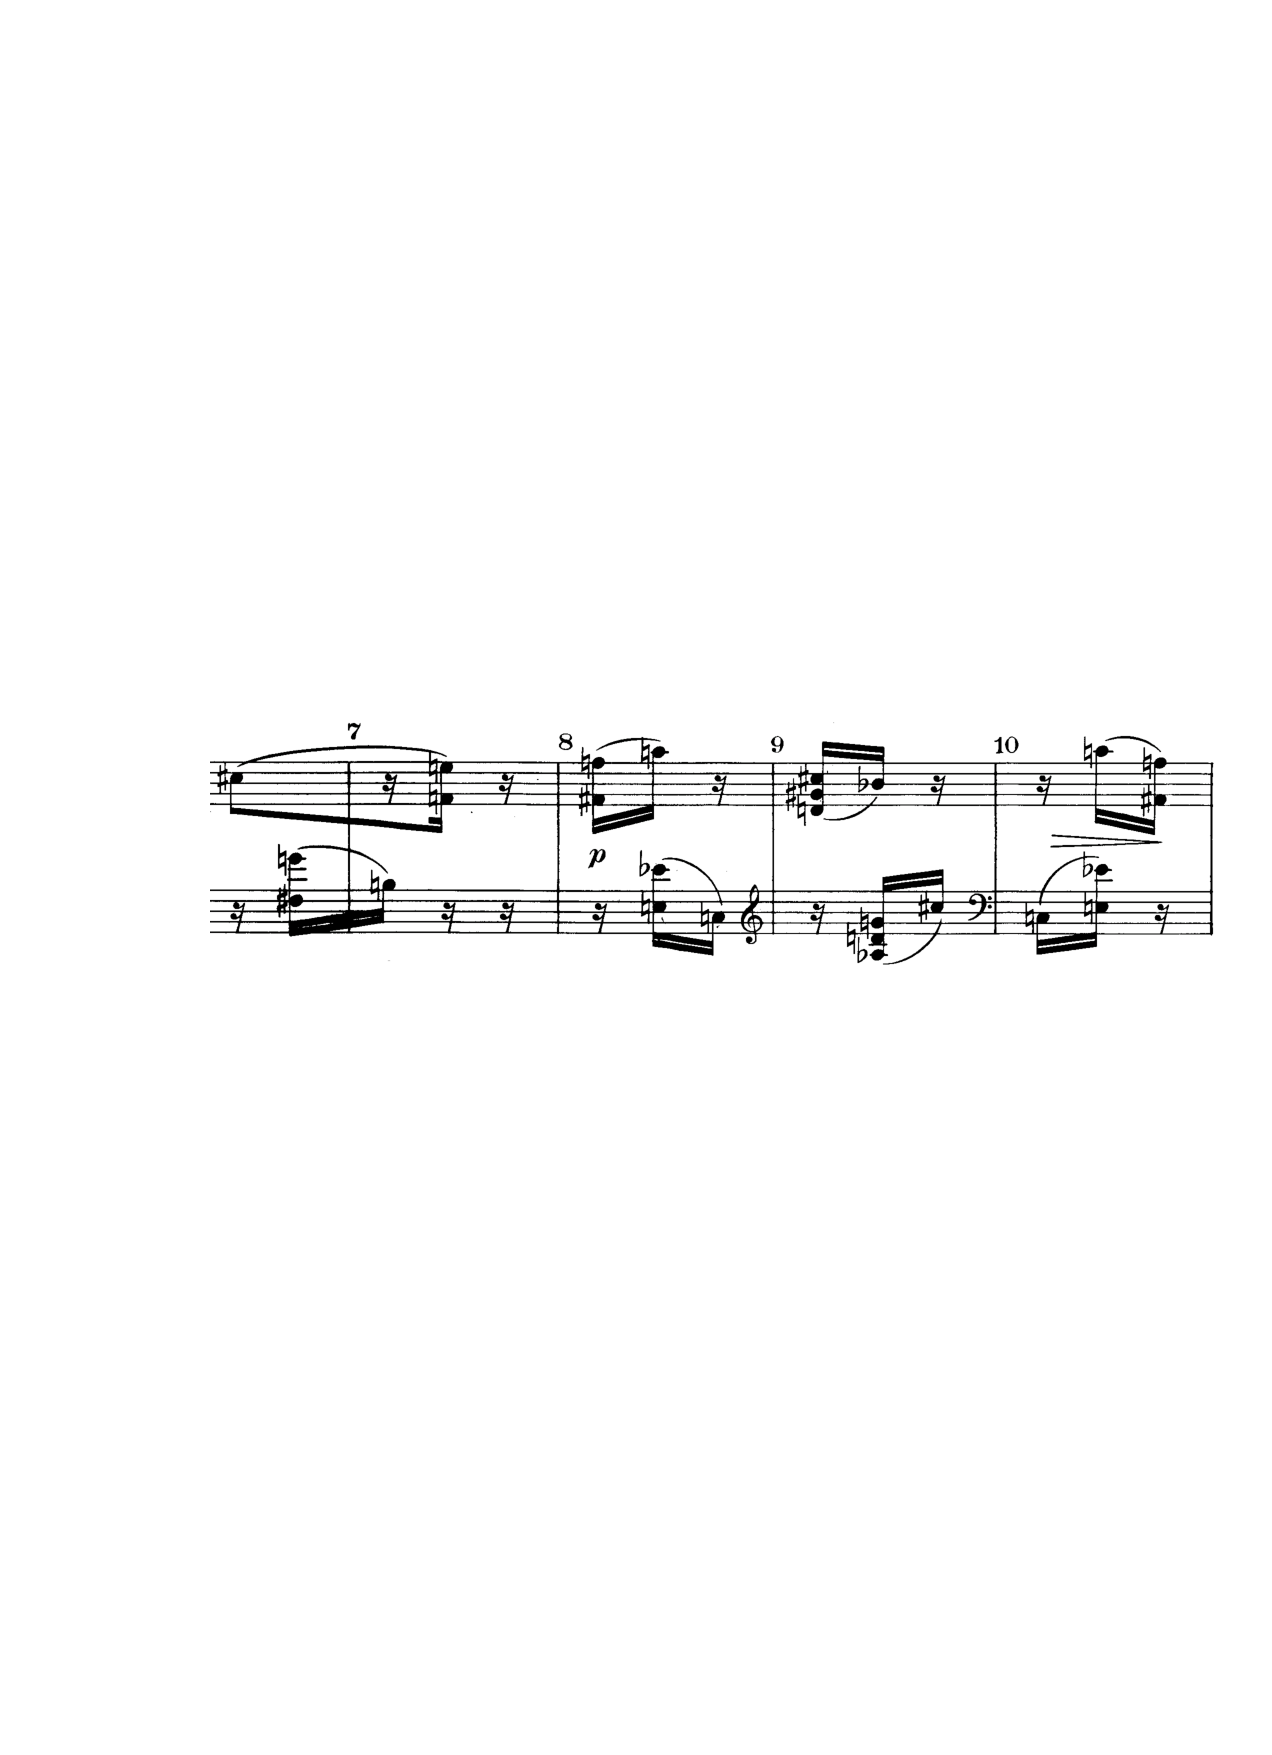
\includegraphics[width=6.5in]{figures/webern2.pdf}
	\caption[Bars 8--10 in Webern's Op.~27]{Bars 8--10 in Webern's Op.~27.}
    \label{fig:webern-27-b}
\end{figure}

\begin{figure}[htbp]
    \centering
	\begin{tikzcd}
	    &&& E\flat \arrow[ddr] &&&& \\
	    & E \arrow[dr] && D \arrow[dr] &&& G \arrow[dr] & \\
	    * \arrow[ur] \arrow[dr] && C\sharp \arrow[ur] \arrow[dr] \arrow[uur] \arrow[ddr] && A \arrow[r] & B\flat \arrow[ur] \arrow[dr] && B \\
	    & F \arrow[ur] && C \arrow[ur] &&& F\sharp \arrow[ur] & \\
	    &&& G\sharp \arrow[uur] &&&&
    \end{tikzcd}
	\caption[An Aggregate Realization of Bars 8--10 in Webern's Op.~27]{We denote the undelying partial order depicted in this aggregate realization by $D_2$.}
    \label{fig:webern-aggregate-c}
\end{figure}

The next excerpt we analyze in the first movement is the last one we need in order to infer what series Webern used for the piece. The musical passage taken from bars 19--23 is given in Fig.~\ref{fig:webern-27-c}, and an aggregate realization is displayed in Fig.~\ref{fig:webern-aggregate-d}. We again normalize it with respect to $S$. This time, the series we are looking for in the excerpt is $\T_3\I(S) = \{ 11, 10, 2, 0, 3, 1, 7, 6, 5, 9, 8, 4 \}$, and again it has a very convoluted presentation, floating around in register, and freely changing hands. We come to the realization that, without the score, it is unlikely that a listener, even a very educated one, will likely be able to discern the composer's main generative material in one hearing. That well-versed listener might not be able to discern it in the hundredth hearing, we even suspect. We shall conclude the analysis before come back to this discussion, however.

\begin{figure}[htbp]
    \centering
	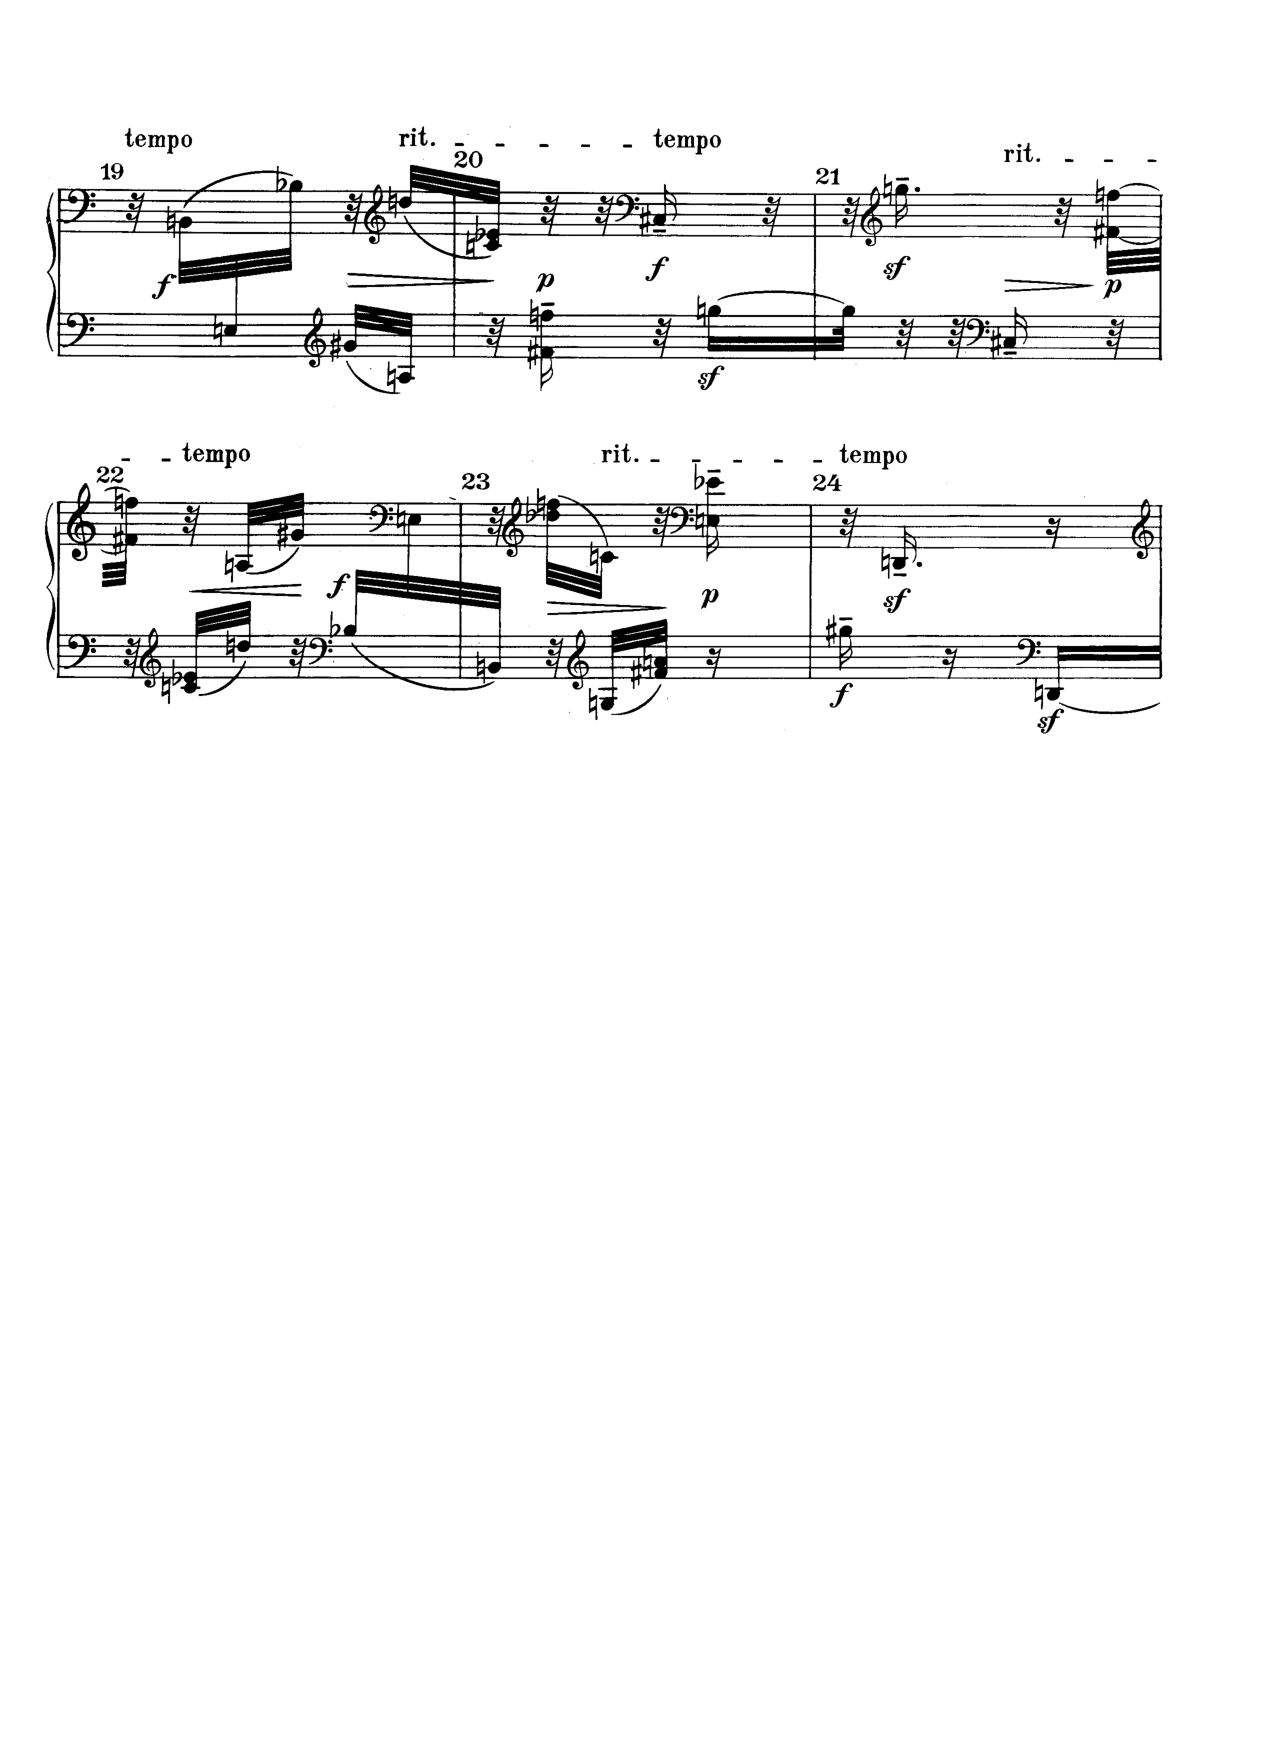
\includegraphics[width=6.5in]{figures/webern3.pdf}
	\caption[Bars 19--23 in Webern's Op.~27]{Bars 19--23 in Webern's Op.~27.}
    \label{fig:webern-27-c}
\end{figure}

\begin{figure}[htbp]
    \centering
	\begin{tikzcd}
	    & [-1em] & [-1em] & [-1em] E\flat \arrow[dr] & [-1em] & [-1em] & [-1em] B\flat \arrow[dr] & [-1em] & [-1em] & [-1em] \\
	    E \arrow[r] & [-1em] F \arrow[r] & [-1em] C\sharp \arrow[ur] \arrow[dr] & [-1em] & [-1em] D \arrow[r] & [-1em] G\sharp \arrow[ur] \arrow[dr] & [-1em] & [-1em] F\sharp \arrow[r] & [-1em] G \arrow[r] & [-1em] B \\
	    & [-1em] & [-1em] & [-1em] C \arrow[ur] & [-1em] & [-1em] & [-1em] A \arrow[ur] & [-1em] & [-1em] & [-1em]
    \end{tikzcd}
	\caption[An Aggregate Realization of Bars 19--23 in Webern's Op.~27]{We denote the undelying partial order depicted in this aggregate realization by $D_3$.}
    \label{fig:webern-aggregate-d}
\end{figure}

The last step in figuring out Webern's total order, according to our theoretical assumptions so far, is to take intersections of the partial orders depicted above with aggregate realizations. Assuming one could actually hear the actual presentation of the series without being victimized by any of the inumerous pitfalls represented by all the registral displacements in the piece, and furthermore assuming one could freely invert and transpose twelve ordered and different pitch classes in their heads almost instantly, one would possibly arrive with the intersection $D_1 \cap D_2$ at measure 10. An aggregate realization of the intersection is shown in Fig.~\ref{fig:webern-aggregate-e}. One would still be puzzled, however, since there are still three incomparabilities that prevent one from comprehending the underlying series.

\begin{figure}[htbp]
    \centering
	\begin{tikzcd}
	    & [-1em] E \arrow[dr] & [-1em] & [-1em] & [-1em] D \arrow[dr] & [-1em] & [-1em] & [-1em] & [-1em] G \arrow[dr] & [-1em] \\
	    * \arrow[ur] \arrow[dr] & [-1em] & [-1em] C\sharp \arrow[r] & [-1em] E\flat \arrow[ur] \arrow[dr] & [-1em] & [-1em] G\sharp \arrow[r] & [-1em] A \arrow[r] & [-1em] B\flat \arrow[ur] \arrow[dr] & [-1em] & [-1em] B \\
	    & [-1em] F \arrow[ur] & [-1em] & [-1em] & [-1em] C \arrow[ur] & [-1em] & [-1em] & [-1em] & [-1em] F\sharp \arrow[ur] & [-1em] \\
    \end{tikzcd}
	\caption[Intersecting Bars 1--7 with Bars 8--10 in Webern's Op.~27]{The intersection $D_1 \cup D_2$.}
    \label{fig:webern-aggregate-e}
\end{figure}

The next two pictures depict aggregate realizations for the intersections $D_1 \cap D_3$ and $D_2 \cap D_3$. Having reached measure 23, we are finally in a position to obtain Webern's series. Both intersections, however, still carry incomparabilities, so we will only be able to achieve our goal by taking the intersection of all three aggregate realizations.

\begin{figure}[htbp]
    \centering
	\begin{tikzcd}
	    & [-1em] & [-1em] & [-1em] & [-1em] & [-1em] & [-1em] & [-1em] B\flat \arrow[dr] & [-1em] & [-1em] & [-1em] \\
	    E \arrow[r] & [-1em] F \arrow[r] & [-1em] C\sharp \arrow[r] & [-1em] E\flat \arrow[r] & [-1em] C \arrow[r] & [-1em] D \arrow[r] & [-1em] G\sharp \arrow[ur] \arrow[dr] & [-1em] & [-1em] F\sharp \arrow[r] & [-1em] G \arrow[r] & [-1em] B \\
	    & [-1em] & [-1em] & [-1em] & [-1em] & [-1em] & [-1em] & [-1em] A \arrow[ur] & [-1em] & [-1em] & [-1em]
    \end{tikzcd}
	\caption[Intersecting Bars 1--7 with Bars 19--23 in Webern's Op.~27]{The intersection $D_1 \cup D_3$.}
    \label{fig:webern-aggregate-f}
\end{figure}

\begin{figure}[htbp]
    \centering
	\begin{tikzcd}
	    & [-1em] & [-1em] & [-1em] E\flat \arrow[dr] & [-1em] & [-1em] & [-1em] & [-1em] & [-1em] & [-1em] & [-1em] \\
	    E \arrow[r] & [-1em] F \arrow[r] & [-1em] C\sharp \arrow[ur] \arrow[dr] && [-1em] D \arrow[r] & [-1em] G\sharp \arrow[r] & [-1em] A \arrow[r] & [-1em] B\flat \arrow[r] & [-1em] F\sharp \arrow[r] & [-1em] G \arrow[r] & [-1em] B \\
	    & [-1em] & [-1em] & [-1em] C \arrow[ur] & [-1em] & [-1em] & [-1em] & [-1em] & [-1em] & [-1em] & [-1em]
    \end{tikzcd}
	\caption[Intersecting Bars 8--10 with Bars 19--23 in Webern's Op.~27]{The intersection $D_2 \cup D_3$.}
    \label{fig:webern-aggregate-g}
\end{figure}

It is with bitter-sweet joy that we finally declare victory in Fig.~\ref{fig:webern-aggregate-h}, as we know we would not stand a chance relying on hearing alone.

\begin{figure}[htbp]
    \centering
	\begin{tikzcd}
	    E \arrow[r] & [-1em] F \arrow[r] & [-1em] C\sharp \arrow[r] & [-1em] E\flat \arrow[r] & [-1em] C \arrow[r] & [-1em] D \arrow[r] & [-1em] G\sharp \arrow[r] & [-1em] A \arrow[r] & [-1em] B\flat \arrow[r] & [-1em] F\sharp \arrow[r] & [-1em] G \arrow[r] & [-1em] B
    \end{tikzcd}
	\caption[The intersection of Bars 1--7, 8--10, and 19--23 in Webern's Op.~27]{The intersection $D_1 \cup D_2 \cup D_3$.}
    \label{fig:webern-aggregate-h}
\end{figure}

\end{example}

There is much to say about Ex.~\ref{starr-webern-example}.

%--------------------------------------------------------------------------
\newpage
\section{The Mallalieu Property}

Consider the 12-tone series $S = \{ 0, 1, 4, 2, 9, 5, 11, 3, 8, 10, 7, 6 \}$. This series has the remarkable property that, if we include a dummy $13^\text{th}$ element, then taking every $n^\text{th}$ element of $S$ produces a transposition of it.

\begin{example}
	We have $S^* = \{ 0, 1, 4, \dots, 7, 6, * \}$. Then taking every zeroth order number of $S^* \mod 13$ yields $S^*$ itself. Taking every first order number yields the series $\{ 1, 2, 5, \dots, 8, 7, * \}$ which, upon removing the dummy symbol, becomes $\T_1 \circ S$. Repeating this procedure every $n^\text{th}$ order number gives the sequence of transforms $\{ \T_i \}_{i \in S}$.
\end{example}

This most peculiar property, commonly called the \emph{mallalieu} property, was first discovered by Pohlman Mallalieu \cite[285]{Lewin1966}. It is natural to ask at this point how many different 12-tone rows are there sharing this property. Unfortunately, there is only one such 12-tone row class under $\T_n\M\I$. We phrase below a little differently an argument given in \cite[17]{Morris1976}.

\cite[278]{Lewin1966} provides a way of looking at mallalieu rows from the standpoint of replacing, for any 12-tone row, its order-number row $\{ 0, 1, \dots, 11 \}$ by the array of integers $\{ 1, 2, \dots, 12, 0 \}$ modulo 13. It is easy to see that such an array has the same structure as the array $S_*$ we constructed above if we substitute the asterisk by the number 12 and consider multiplication as the group operation. Obviously, this is just the isomorphism between the integers modulo 12 and the group of units modulo 13. One of the advantages of this approach is that we can dispense with the extra symbol altogether and just use the indices from 1 to $p - 1$. We shall, however, still refer to the row of order numbers as $S^*$, the context making it clear whether we are constructing it with an asterisk or not. The process of taking every $n^\text{th}$ element of a 12-tone row becomes then just the aforementioned multiplicative group operation on order numbers, that is, multiplying order numbers by $k \pmod{13}$ is the same as taking every $k^\text{th}$ element of a row.

\begin{example}
	Put $S = \{ 0, 1, \dots, 11 \}$ and $S^* = \{ 1, 2, \dots, 12 \}$. Then
	\begin{equation}
		\M_3 \circ S^* = \{ 3, 6, \dots, 10 \} \enspace,
	\end{equation}
	which corresponds to the row $R = \{ 2, 5, \dots, 9 \}$. The row $R$ can be equivalently constructed by placing an asterisk as the $13^\text{th}$ order number of $S$ and taking every third element. The fact that $R$ and $S$ are not related by $\T_n\M\I$ reflects the fact that neither $S$ nor $R$ have the mallalieu property.
\end{example}

It should be of interest to many composers whether other $n$-TET systems are capable of producing mallalieu rows, and if so, how many. Unfortunately, answering this question is not as straightforward as the above discussion, since we can no longer rely on the isomorphism that constitutes the proof of \ref{lewin-mallalieu}. We shall reformulate this question at the end of the present chapter, after having covered more of what has been already done.

If, on one hand, we only get one $\T_n\M\I$ row class with the mallalieu property in 12 tones, we do get considerably more row classes when we relax the requirement that a row produce a transposition of itself when taking every $n^\text{th}$ of its elements. This idea is explored in part by \cite{Mead1989}, however without specifying any combinatorial aspect (in the mathematical sense) of this generalization. Moreover, we can certainly go beyond \cite{Mead1989} and investigate, in 12 tones, what an extension of the mallalieu property could yield under operations other than transposition.
